%   File: ski_jumper.tex
% Author: Adam Leeper
%------------------------------------------------------------------------------
%\\[0.45pc]
\providecommand{\isolatedBuild}[1]{#1}% fallback definition lets this file build normally
\isolatedBuild{
  \documentclass[11pt,letterpaper]{book}
  %\documentclass[11pt,letterpaper]{book}

% aleeper: I think these are needed for Paul's macros?
\usepackage{epsfig}
\usepackage{epstopdf}

%\makeatletter
%\typeout{The import path is \import@path}
%\makeatother

\usepackage{import}

\subimport{./}{packagesMitiguy.sty}
\subimport{./}{macrosMitiguy.tex}
\subimport{./}{PageStylesMitiguy.tex}
\subimport{./}{macrosLeeper.tex}
   % Must be found via TEXINPUTS environment variable.
  \isolatedBuildHeader{Projectile Motion Examples}
                      {Projectile Motion of a Ski Jumper\footnote{Answer: d = 21.28 m, perpendicular speed = 6.87 m/s, total speed = 21.3 m/s.\\[0.0pc]
This is adapted from Example 13.7 from Bedford \& Fowler, Engineering Mechanics Dynamics, 3rd ed., Prentice Hall, 2002.}}
}
%%%
%%%
%%%
\small
\begin{minipage}[t]{0.57\textwidth}
A skier launches from the $\degrees{20}$ slope with an initial speed of 10 m/s.
%Using $g = 9.81$ m/s$^2$ for the gravitational constant,
\begin{enumerate}
\item Find the landing distance $d$ along the lower slope.
\item Find the component of the skier's speed perpendicular to the lower slope immediately prior to landing (this affects leg impact).
\item Find  of his total speed immediately prior to landing.
\end{enumerate}
\vspace{0.5pc}
As a suggestion, introduce labels for points of interest in the world
and introduce unit vectors that make it easy to express the quantities in the problem.
Then, introduce scalar variables for the skier's position as measured from some point, and pick them to be measured along unit vectors that make the math easiest.
%
\\[0.5pc]\textbf{Hint:} \underline{Don't} pick horizontal and vertical measures.
\end{minipage}
\hfill
\begin{minipage}[t]{0.35\textwidth}
\vspace*{-2.0pc}
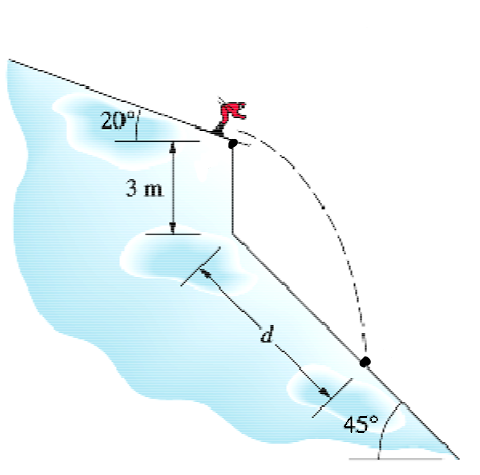
\includegraphics[width=1.0\textwidth]{ski_jump.png}
\end{minipage}

In general, projectile motion problems require you to identify relevant position scalars for the projectile, and then to find a set of differential equations for those variables.
Examples in most textbooks pick horizontal and vertical measures by default.
However, doing this on ``sloped'' problems often requires additional variables or potentially tricky algebraic substitutions.
Instead, we'll use the power of dot products and rotation tables to simplify our book-keeping by introducing unit vectors as needed.
%
\section*{MIPSI Process:}
\subsection*{Modeling}
Our modeling assumptions include
taking the earth to be a Newtonian reference frame,
neglecting air resistance,
modeling the skier as a particle,
and assuming a uniform gravitational field throughout the flight.

\subsection*{Identifiers}
Let the earth be a Newtonian reference frame \basis{N}, and we'll call the particle representing the skier $Q$. Let's label the jumping point $N_1$, and the point vertically below it (where the landing distance is measured from) $N_2$. We know that we will need to describe a vertically-downward gravitational force, so we'll introduce a set of orthogonal unit-vectors \uvecxyz{n} as shown. Next, the initial velocity $\vel{Q}{N}_i$ is along the $\degrees{20}$ slope, so we'll go ahead and introduce orthogonal unit-vectors \uvecxyz{a} as shown. Finally, since we care about the landing distance along the lower slope we'll introduce orthogonal unit-vectors \uvecxyz{b} as shown. Note that while we might refer to the existence of a rigid frame \basis{A} or \basis{B}, their respective unit vectors are really just additional bases \textbf{fixed} in \basis{N}.
%In other words, since frames \basis{A} and \basis{B} are fixed in \basis{N}, \textbf{all unit vectors are fixed in \basis{N}}.
\\[0.5pc]
Picking the right position scalars can make the difference between this problem being easy or hard.
We could measure $Q$'s position from $N_1$ or from $N_2$, and we could measure it along any of the unit vectors we have introduced. Based on what we are trying to find, the easiest way (in my opinion) is to measure the position from $N_2$, \textit{along} the \uvecx{b} and \uvecy{b} directions. We'll call the measures $x$ and $y$, hence, $\posvec{N_2}{Q} \equals[\;] x~\uvecx{b} + y~\uvecy{b}$.
\\[0.5pc]
The advantage of this parametrization is that it makes it really easy to determine $d$ (it is just $x$), and it is also straight-forward to determine when the skier hits the slope (when $y < 0$). If the position scalars were measured along \uvecx{n} and \uvecy{n} then the condition for the skier hitting the lower slope would be a function of $y$ \textit{and} $x$, which would require additional algebraic cleverness.
%
\subsection*{Physics}
Since we care about the translational position of $Q$, we will use $\force{Q} = m^Q * \accel{Q}{N}$ to solve this problem (we will eventually use the ``Roadmap" method from section 20.7 to help make this more obvious).
\\[0.5pc]
\textbf{\underline{Kinematics:}} First we'll find a way to describe the \textit{motion} of $Q$.
$$\posvec{N_2}{Q} \equals[\;] x~\uvecx{b} + y~\uvecy{b}$$
$$\vel{Q}{N} ~\deff~ \dt[N]{}(\posvec{N_2}{Q}) \equals[\;] \xdot~\uvecx{b} + \ydot~\uvecy{b} $$
\begin{equation}
\accel{Q}{N} ~\deff~ \dt[N]{}(\vel{Q}{N}) \equals[\;] \xddot~\uvecx{b} + \yddot~\uvecy{b}
\end{equation}
Note that \textbf{in this case} the golden-rule is not needed since \uvecx{b} and \uvecy{b} are fixed in \textbf{N}.
\\[1.0pc]
\textbf{\underline{Forces:}}
Next we'll write down all the \textit{contact} and \textit{distance} forces on $Q$.
\begin{equation}
\force{Q} = \bvec{F}_\mathrm{gravity} + \bvec{F}_\mathrm{unmodeled} = m^Q*g~(-\uvecy{n})
\end{equation}
\\[0.5pc]
\textbf{\underline{Applying Laws of Motion:}}
We are now allowed to use equations (1) and (2) as
\textit{ingredients} in $\force{Q} = m^Q * \accel{Q}{N}$:
\begin{equation}
-m^Q*g~\uvecy{n} \equals[\;] m^Q * (\xddot~\uvecx{b} + \yddot~\uvecy{b})
\end{equation}
\begin{equation}
-g~\uvecy{n} \equals[\;] \xddot~\uvecx{b} + \yddot~\uvecy{b}
\end{equation}
Notice that the mass of the projectile always cancels out in projectile motion problems with \textit{only} gravity forces.
\\[1.0pc]
\textbf{\underline{Getting Differential Equations:}}
We want differential equations for $\xddot$ and $\yddot$, so let's dot with \uvecx{b} and \uvecy{b}.
\begin{equation}
g~\sin(\degrees{45}) \equals[\;] \xddot
\end{equation}
\begin{equation}
-g~\cos(\degrees{45}) \equals[\;] \yddot
\end{equation}
\subsection*{Solve}
We can integrate the differential equations by hand/numerically, or notice that both differential equations say that the 2nd-derivative of a variable is \textit{constant}. Hence, we can also apply the equations in section 8.3. In either case, we still need to find the initial conditions for $\xdot$, $\ydot$, $x$, and $y$.
%
\\[0.5pc]The initial velocity can be written
$\vel{Q}{N}_i \equals[\;] 10\frac{\mathrm{m}}{\mathrm{s}}~\uvecx{a} \equals[\;] \xdot_i~\uvecx{b} + \ydot_i~\uvecy{b}$.
Dotting both sides with \uvecx{b} and \uvecy{b} yields
$$\xdot_i = 10 \cos(\degrees{25}) ~\mathrm{m/s}$$
$$\ydot_i = 10 \sin(\degrees{25}) ~\mathrm{m/s}$$
%
\\[0.5pc]The initial position can be written
$\posvec{N_2}{N_1} \equals[\;] 3~\uvecy{n} \equals[\;] x_i~\uvecx{b} + y_i~\uvecy{b}$.
Dotting both sides with \uvecx{b} and \uvecy{b} yields
$$x_i = -3 \sin(\degrees{45}) ~\mathrm{m}$$
$$y_i =  3 \cos(\degrees{45}) ~\mathrm{m}$$
%
\\[0.5pc]
With the initial conditions in-hand we can now solve. The end of the jump is defined as the instant the skier touches down on the slope, so we need to find the \textit{time} until $y = 0$.
Using $s - s_i = v_i t + \frac{1}{2} a t^2$ we have:
$$0 - 3 \cos(\degrees{45}) \equals[\;] 10 \sin(\degrees{25}) ~ t
\plus[\;]\frac{1}{2} ( -g~\cos(\degrees{45})) ~ t^2 $$
%
Solving for $t$ yields $t = -0.382$ or $t = 1.6$ seconds. The physically meaningful solution is the positive root.
\\[0.0pc]Now we can find $x$ using the same equation:
$$x - (-3 \sin(\degrees{45})) \equals[\;] 10 \cos(\degrees{25}) ~ (1.6)
\plus[\;] \frac{1}{2} (g~\sin(\degrees{45})) ~ (1.6)^2 $$
%
Solving yields $x = 21.28$ meters.
\\[0.5pc]
\textbf{\underline{Speed:}} Since we already solved for $t$ at the time of impact, we can use the equation $v_f = v_i + at$ for both $\xdot$ and $\ydot$:

$$\xdot_f \equals[\;] 10~\cos(\degrees{25}) \plus[\;] (g \sin(\degrees{45})*(1.6) \equals[\;] 20.16 ~\mathrm{m/sec}$$
$$\ydot_f \equals[\;] 10~\sin(\degrees{25}) \minus[\;] g \cos(\degrees{45})*(1.6) \equals[\;] -6.87 ~\mathrm{m/sec}$$

\subsection*{Interpret}
We were originally asked for a distance $d$ from the top of the lower slope.
Since we chose our identifiers well, the result is just $d = x = 21.28$ meters.
\\[0.5pc]
We were also asked for the skier's speed perpendicular to the slope when he lands, which is $\magnitude{\ydot_f} \equals[\;] 6.87 ~\mathrm{m/sec}$.
His total speed is
$\magnitude{\vel{Q}{N}_f} \equals[\;] \magnitude{\xdot_f~\uvecx{b} \plus[\;] \ydot_f~\uvecy{b}}
\equals[\;] \sqrt{\xdot_f^2 \plus[\;] \ydot_f^2}
 \equals[\;] 21.3 ~\mathrm{m/sec}$.


\section*{Numerical/Graphical Solution}
The MotionGenesis code on the next page simulates the ski jump by integrating the differential equations numerically. Inspection of the graph shows the same result of $x = 21.28$ meters when $y = 0$.
\\[1.0pc]
\begin{center}
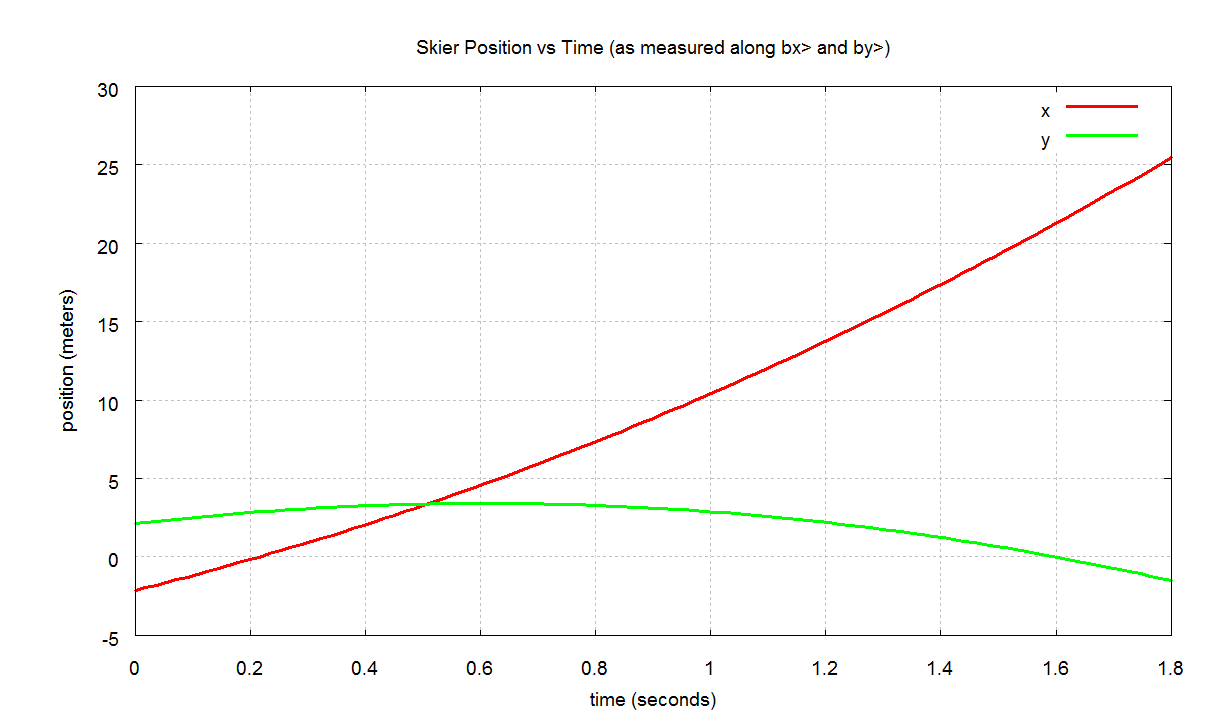
\includegraphics[width=0.8\textwidth]{skier.png}
\end{center}
\vfill
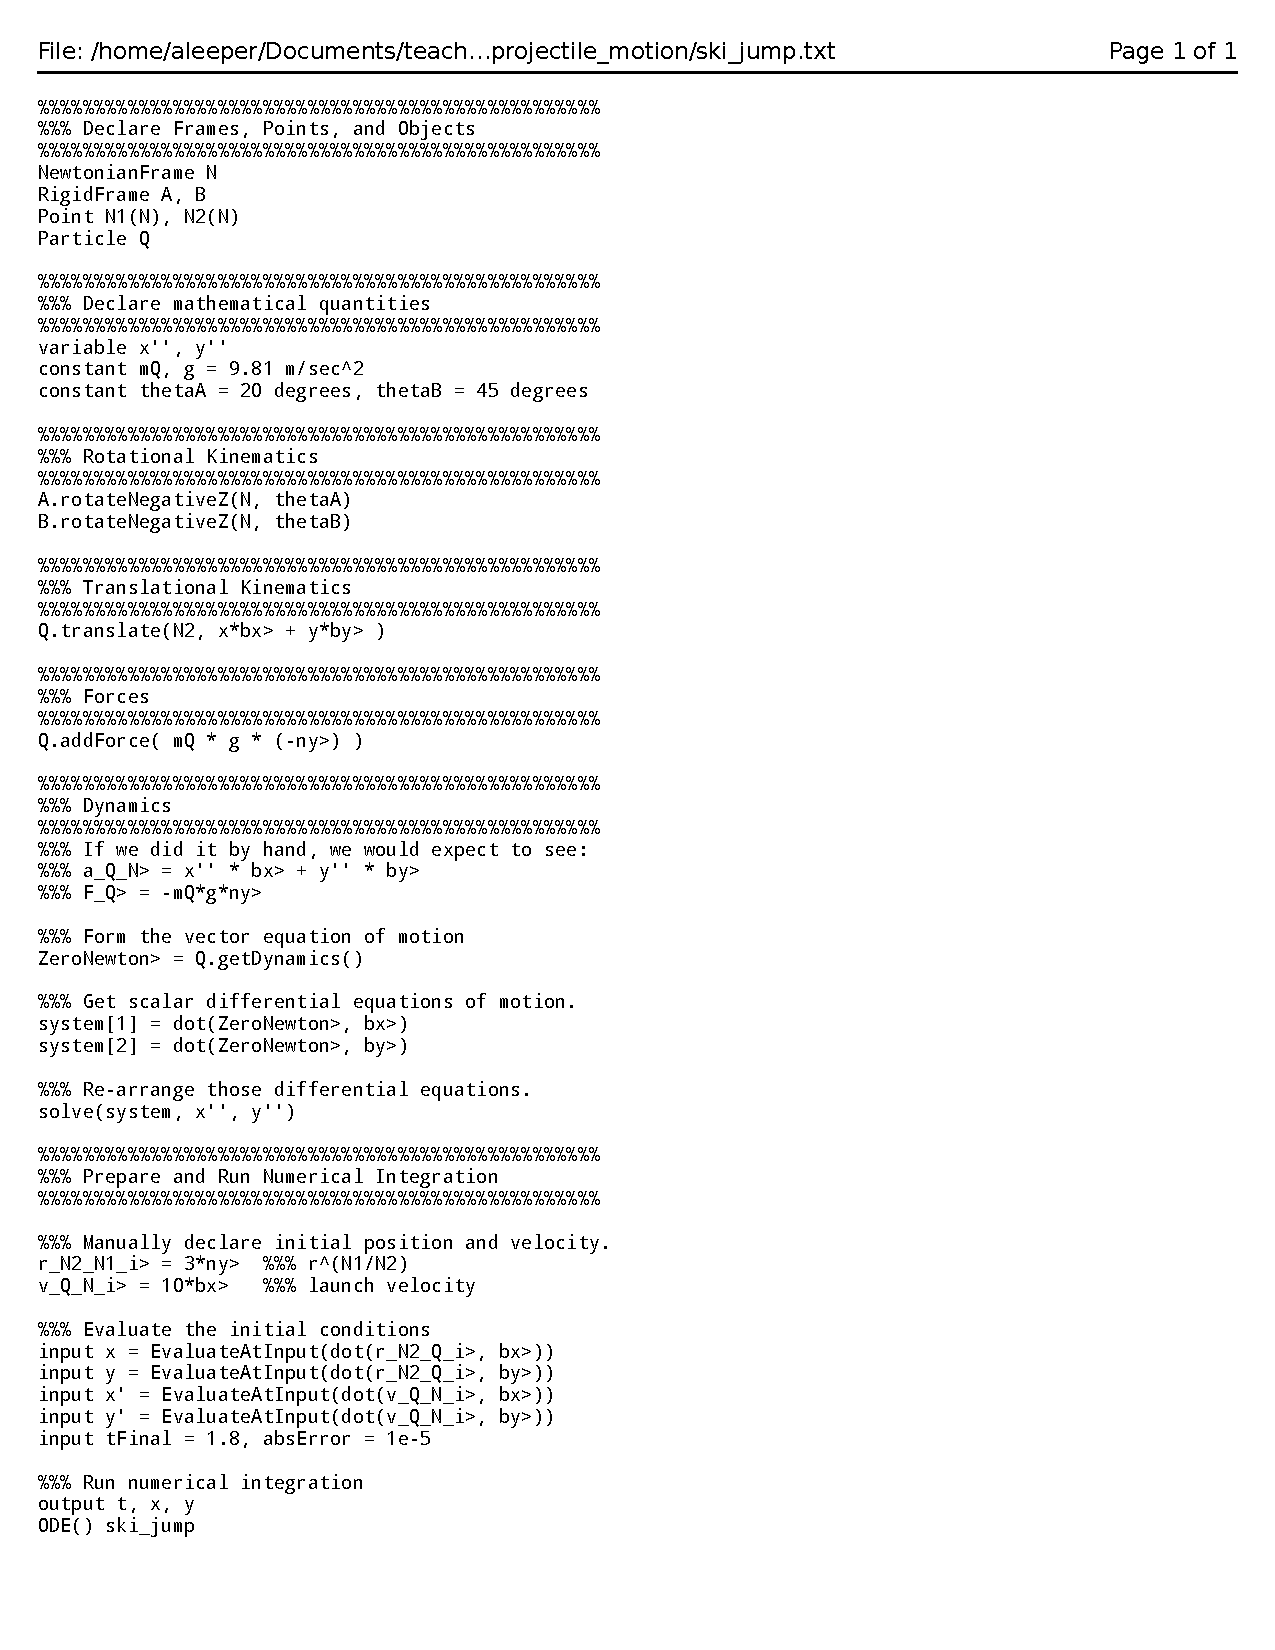
\includegraphics[scale=0.9]{skier_mg.pdf}
\vfill
%}  % end solution
%
\isolatedBuildFooter
